% ============================================================================
%  Exact exponential heat rectification from the Liouvillian skin effect
%  Target: Physical Review Letters (revtex4-2, reprint, aps, prl)
%  Figures are generated from ../results/*.json by make_figures.py.
% ============================================================================
\documentclass[reprint,aps,prl,superscriptaddress,nofootinbib,floatfix]{revtex4-2}
\usepackage{amsmath,amssymb,bm}
\usepackage{graphicx}
\graphicspath{{figures/}}
\usepackage[colorlinks=true,linkcolor=blue,citecolor=blue,urlcolor=blue]{hyperref}
\usepackage{xcolor}
\newcommand{\R}{\mathcal{R}}
\newcommand{\dQ}{\delta Q}
\newcommand{\heff}{h_{\rm eff}}

\begin{document}

\title{Exact exponential heat rectification from the Liouvillian skin effect}

\author{Hikaru Wakaura}
\altaffiliation{ORCID: 0000-0001-8381-8323}
\email{h.wakaura@qiri.co.jp} 
\affiliation{QIRI (Quantum Integrated Research Institute Inc.), Tokyo 107-0061, Japan}
\author{Taiki Tanimae}
\email{t.tanimae@qiri.co.jp} 
\affiliation{QIRI (Quantum Integrated Research Institute Inc.), Tokyo 107-0061, Japan}


 
 
  
   

\date{\today}

\begin{abstract}
Directing heat is as basic to thermal engineering as directing charge is to electronics, yet every thermal diode to date relies on nonlinearity or structural asymmetry.
Here we show that a reciprocal tight-binding chain with directional bond dissipation rectifies heat with the exact ratio $\dQ_f/\dQ_r=\exp[2(L-1)/\xi]$, where $L$ is the chain length and $\xi$ the Liouvillian skin localisation length, so that forty sites suffice for 99\% rectification.
The law holds at every energy and temperature and for arbitrary on-site disorder; beyond nearest neighbours the exponent is the non-Bloch localisation length, not the spectral winding number, and matrix-product-state simulations show that interactions up to twice the hopping leave the skin length unrenormalised.
A thermal bath in place of the loss closes the entropy balance at a cost per rectified heat that grows with the inverse skin length.
Our results make the Liouvillian skin effect a design principle for size-scalable heat diodes in cold atoms and superconducting circuits.
\end{abstract}

\maketitle

\textit{Introduction.}---Directing heat is as fundamental to thermal engineering as directing charge is to electronics, and a thermal diode is the elementary building block of thermal logic and of heat management in nanoscale devices~\cite{Terraneo2002,Li2004,Chang2006,Li2012,Benenti2017}.
All thermal rectifiers demonstrated so far share one requirement: the two directions of heat flow must probe different energy spectra, which is achieved through anharmonicity, temperature-dependent spectral overlap or structural asymmetry~\cite{Segal2005,Li2012}, and the quantum thermal diodes proposed recently are no exception~\cite{Zhang2025}.
Because these mechanisms act locally, the resulting rectification ratios saturate at values of order one to ten and do not improve with the size of the device.
A qualitatively different source of directionality has emerged in non-Hermitian physics.
Lattices with asymmetric hopping~\cite{Hatano1996} pile all their eigenstates up at one edge, the non-Hermitian skin effect~\cite{Yao2018,Gong2018,Lee2019,Okuma2020,Bergholtz2021}, and the same phenomenon appears in the Liouvillian of an open quantum system whose dissipators carry a direction~\cite{Song2019,Haga2021,Metelmann2015,Rassaert2025,Shigedomi2026}, a directionality that survives dephasing~\cite{Wang2026}.
Skin modes have been observed in photonic, electrical and cold-atom platforms~\cite{Weidemann2020,Helbig2020,Xiao2020,Liang2022,Zhou2025} and even in classical heat diffusion~\cite{Cao2021,Liu2024}, and amplification along a skin lattice has been proposed for sensing~\cite{McDonald2020} and observed in bosonic Kitaev chains~\cite{Busnaina2024,Slim2024}.
However, it is not known whether directional dissipation alone can rectify heat between two thermal reservoirs, what quantity controls the ratio, whether the effect survives interactions and disorder, and what entropy it produces.
Here we answer these questions for the simplest model, a reciprocal fermionic chain with directional bond loss between two leads.
We find that the ratio of the heat-current responses in the two directions obeys an exact law, $\dQ_f/\dQ_r=e^{2(L-1)/\xi}$ with $\xi$ the skin length, for any energy, temperature and on-site disorder; that the controlling quantity beyond nearest neighbours is the energy-resolved non-Bloch localisation length and not a spectral winding number; that a nearest-neighbour interaction leaves $\xi$ unrenormalised; and that the entropic cost per rectified heat grows as $1/\xi$ when the dissipator is a finite-temperature bath.
The result shows that skin-effect rectification is a structural property of one-dimensional dissipative transport and provides a design rule, $L/\xi\gtrsim3$, for near-perfect heat diodes.

\begin{figure*}[t]
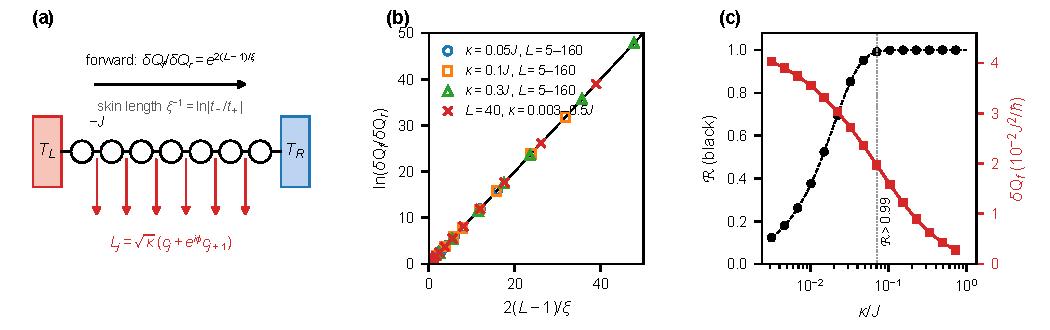
\includegraphics[width=\textwidth]{fig1.pdf}
\caption{\textbf{Heat rectification by directional bond loss obeys the exact law $\dQ_f/\dQ_r=e^{2(L-1)/\xi}$.}
(a) Reciprocal chain (hopping $-J$) between leads at $T_L$ and $T_R$; every bond carries the loss operator $L_j$, which fixes the skin length $\xi^{-1}=\ln|t_-/t_+|$ and favours transport from left to right.
(b) Logarithm of the ratio of the forward and reverse $\Delta T$ responses against $2(L-1)/\xi$ for $\phi=\pi/2$, $T_h=J$, $T_c=0.5J$ and wide-band leads ($\Gamma=J$); all lengths and loss rates fall on the line $y=x$ to machine precision.
(c) Rectification $\R=\tanh[(L-1)/\xi]$ (black, dashed line is the law) and forward throughput $\dQ_f$ (red) against $\kappa$ for $L=40$; $\R>0.99$ is reached at $\kappa\simeq0.07J$ where $\dQ_f$ is still half of its $\kappa\to0$ value.
}
\label{fig1}
\end{figure*}

\textit{Model and observable.}---We consider spinless fermions on an open chain of $L$ sites, $H=-J\sum_{j=1}^{L-1}(c_j^\dagger c_{j+1}+{\rm h.c.})$, whose density matrix obeys a Lindblad equation with one jump operator per bond,
\begin{equation}
L_j=\sqrt{\kappa}\,\bigl(c_j+e^{i\phi}c_{j+1}\bigr),\qquad j=1,\dots,L-1 .
\label{eq:Lj}
\end{equation}
The Hamiltonian is reciprocal; the phase $\phi$ in the dissipator is the only source of directionality.
Equation~(\ref{eq:Lj}) is the chiral-damping dissipator of Song, Yao and Wang~\cite{Song2019} and the standard route to the Liouvillian skin effect~\cite{Haga2021}; it is obtained by coupling two neighbouring sites to a common strongly damped auxiliary mode with a relative coupling phase and eliminating that mode adiabatically~\cite{Metelmann2015}.
Site 1 (site $L$) is coupled to a fermionic lead at temperature $T_L$ ($T_R$) and common chemical potential $\mu=0$, either as a wide-band reservoir of rate $\Gamma$ or as a mesoscopic bath of $K$ modes.
Because the Lindbladian is quadratic, the steady state is Gaussian and all currents follow from a Lyapunov equation for the covariance matrix (Supplemental Material, SM~\cite{SM}, Sec.~S1); single-particle amplitudes propagate with the non-Hermitian matrix
\begin{equation}
\heff=h-\tfrac{i}{2}\textstyle\sum_j \bar l_j\, l_j^{T},\qquad
t_\pm=-J-\tfrac{i\kappa}{2}e^{\pm i\phi},
\label{eq:heff}
\end{equation}
where $l_j$ is the coefficient vector of $L_j$ and $t_+\equiv(\heff)_{j,j+1}$, $t_-\equiv(\heff)_{j+1,j}$ are the two hopping amplitudes. The on-site part of $\heff$ is a uniform loss $-i\kappa$, and the two hopping amplitudes differ in modulus, $|t_\mp|^2=(J\pm\tfrac{\kappa}{2}\sin\phi)^2+\tfrac{\kappa^2}{4}\cos^2\phi$. For $\phi=\pi/2$, $\heff$ is the Hatano--Nelson chain~\cite{Hatano1996} with real asymmetric hoppings $-J\mp\kappa/2$ and a uniform loss; all its right eigenvectors are localised at the right edge with inverse localisation length $\xi^{-1}=\ln|t_-/t_+|\simeq\kappa\sin\phi/J$.

Rectification must be defined with care in a system that also loses energy to the bulk dissipator.
The total heat current into the cold lead contains a $\Delta T$-independent background flowing from both leads into the loss channel, and a ratio of total currents is dominated by this background and decays as $1/L$ even though the device is perfectly directional.
We therefore use the response of the cold lead to heating the other lead:
$\dQ_f$ is the additional heat absorbed by the right lead when the left lead is heated from $T_c$ to $T_h$, and $\dQ_r$ the additional heat absorbed by the left lead when the right lead is heated. We quote $\R=(|\dQ_f|-|\dQ_r|)/(|\dQ_f|+|\dQ_r|)$ and the ratio $\dQ_f/\dQ_r$. In the wide-band limit both responses take the Landauer form $\dQ_{f,r}=\int\frac{d\varepsilon}{2\pi}\,\varepsilon\,T_{RL,LR}(\varepsilon)[f_h(\varepsilon)-f_c(\varepsilon)]$ with $T_{RL}=\Gamma^2|G_{L1}|^2$ and $T_{LR}=\Gamma^2|G_{1L}|^2$, where $G=(\varepsilon-\heff)^{-1}$ (SM, Sec.~S1).

\textit{Exact law.}---The proof is one line. Since $\heff$ is tridiagonal, the cofactor expansion of $G$ gives $G_{L1}/G_{1L}=\prod_{j=1}^{L-1}(\heff)_{j+1,j}/(\heff)_{j,j+1}=(t_-/t_+)^{L-1}$, independent of $\varepsilon$ and of every diagonal element of $\heff$. Hence
\begin{equation}
\frac{T_{RL}(\varepsilon)}{T_{LR}(\varepsilon)}=\frac{\dQ_f}{\dQ_r}=\Bigl|\frac{t_-}{t_+}\Bigr|^{2(L-1)}\equiv e^{2(L-1)/\xi},
\label{eq:law}
\end{equation}
and therefore $\R=\tanh[(L-1)/\xi]$. The ratio of the energy-resolved transmissions is a constant, so the ratio of their thermal averages is the same constant for any pair of lead distributions, Fermi or Bose, at any temperatures and chemical potentials, and for any on-site potential $\varepsilon_j$, random or not.
Figure~\ref{fig1}(b) confirms Eq.~(\ref{eq:law}) to all digits for $L=5$--$160$ and $\kappa=0.003J$--$0.5J$, a scaling collapse of all lengths and loss rates onto one line, and Fig.~\ref{fig1}(c) shows the design trade-off: $\R$ exceeds $0.99$ once $(L-1)/\xi>2.6$, i.e.\ $L/\xi\gtrsim3$, whereas the forward throughput decreases with $\kappa$ because the same loss that creates the skin effect removes energy from the chain; at $\kappa=0.07J$ and $L=40$ one has $\R=0.992$ with $\dQ_f$ equal to $49\%$ of its lossless value.
Equation~(\ref{eq:law}) is odd in $\phi$ and vanishes identically at $\phi=0,\pi$, where the dissipator is mirror symmetric. Adding bond gain of the same chirality adds to $\kappa$ in $\heff$ and shortens $\xi$ without altering the form of the law (SM, Sec.~S2).

\begin{figure*}[t]
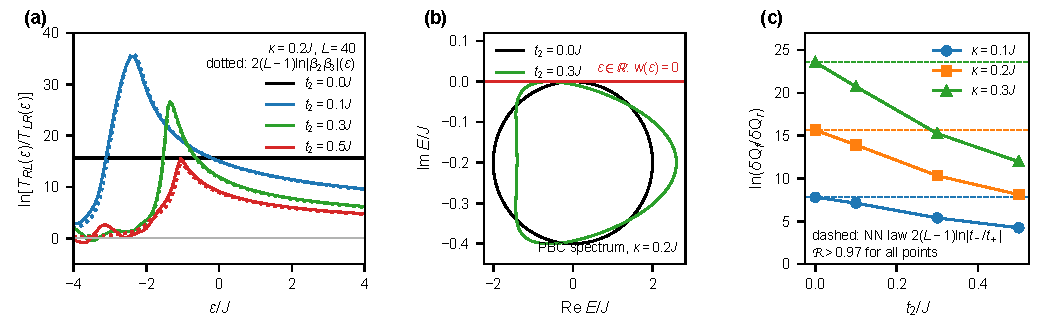
\includegraphics[width=\textwidth]{fig2.pdf}
\caption{\textbf{Beyond nearest neighbours the rectification exponent is the energy-resolved non-Bloch localisation length, not the spectral winding number.}
(a) Logarithmic transmission asymmetry against energy for a reciprocal next-nearest-neighbour hopping $t_2$ ($\kappa=0.2J$, $L=40$, $\phi=\pi/2$); solid lines are exact, dotted lines are $2(L-1)\ln|\beta_2\beta_3|(\varepsilon)$ from the roots of Eq.~(\ref{eq:nonbloch}). For $t_2=0$ the asymmetry is the constant of Eq.~(\ref{eq:law}).
(b) Periodic-boundary spectrum of $\heff$ in the complex plane; the loop touches the real axis at a single point, so the winding number around every transport energy $\varepsilon\in\mathbb{R}$ is zero for all $t_2$.
(c) Thermally averaged ratio $\ln(\dQ_f/\dQ_r)$ against $t_2$; the nearest-neighbour law (dashed) is an upper bound and the rectification remains above $0.97$ for all points.
}
\label{fig2}
\end{figure*}

\textit{What controls the exponent.}---Equation~(\ref{eq:law}) relies on tridiagonality. Adding a reciprocal next-nearest-neighbour hopping $t_2(c_j^\dagger c_{j+2}+{\rm h.c.})$ breaks it and makes the transmission asymmetry strongly energy dependent [Fig.~\ref{fig2}(a)]: it peaks near the lower band edge, decreases monotonically at high energy, and for $t_2\gtrsim0.3J$ even changes sign in a narrow window.
The non-Bloch band theory of the skin effect~\cite{Yao2018,Yokomizo2019} explains this quantitatively. Writing bulk solutions of $\heff\psi=\varepsilon\psi$ as $\psi_j=\beta^j$ gives the characteristic equation
\begin{equation}
t_2\beta^2+t_+\beta-i\kappa-\varepsilon+t_-\beta^{-1}+t_2\beta^{-2}=0,
\label{eq:nonbloch}
\end{equation}
whose four roots, ordered as $|\beta_1|\le|\beta_2|\le|\beta_3|\le|\beta_4|$, satisfy $\beta_1\beta_2\beta_3\beta_4=1$. The transmission asymmetry of a long chain is governed by the two roots that build the generalised Brillouin zone, $\ln[T_{RL}/T_{LR}](\varepsilon)=2(L-1)\ln|\beta_2\beta_3|(\varepsilon)+O(1)$, which reproduces the exact curves for all $t_2$ and $\kappa$ [dotted lines in Fig.~\ref{fig2}(a)]; for $t_2=0$ the product $\beta_1\beta_2=t_-/t_+$ is constant and Eq.~(\ref{eq:law}) is recovered (SM, Sec.~S3).
The thermally averaged ratio therefore becomes the Fermi-window average of an energy-resolved skin length $\xi(\varepsilon)^{-1}=\ln|\beta_2\beta_3|(\varepsilon)$, and it lies below the nearest-neighbour value [Fig.~\ref{fig2}(c)], for example $15.65\to8.11$ at $\kappa=0.2J$ when $t_2$ grows from $0$ to $0.5J$, while $\R$ stays above $0.97$.
This identifies the correct indicator of thermal nonreciprocity. The spectral winding number around a reference energy, which is the usual topological marker of the skin effect~\cite{Gong2018,Okuma2020,Zhang2020}, vanishes at every real transport energy because the periodic-boundary spectrum of $\heff$ has imaginary part $-\kappa(1-\sin k)\le0$ and touches the real axis only at a point [Fig.~\ref{fig2}(b)].
The chain rectifies although $w(\varepsilon)=0$: what matters is the radius ratio of the generalised Brillouin zone at the transport energy, not the winding of the spectrum.

\begin{figure*}[t]
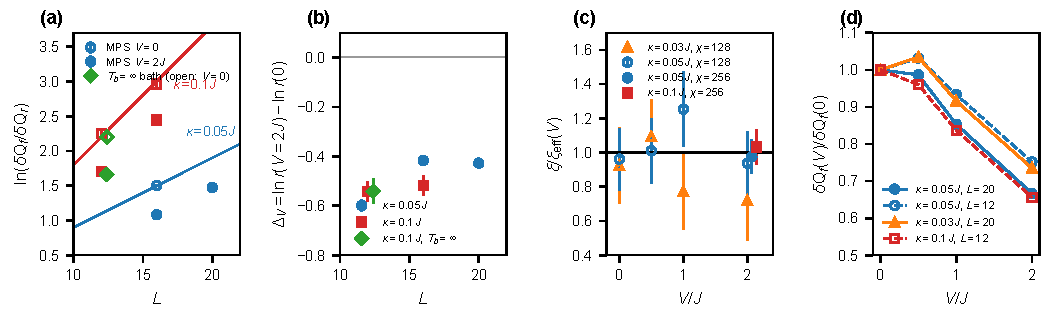
\includegraphics[width=\textwidth]{fig3.pdf}
\caption{\textbf{A nearest-neighbour interaction does not renormalise the skin length and acts as a length-independent prefactor.}
Superfermion matrix-product-state steady states with mesoscopic leads ($K=10$ modes, bandwidth $4J$), $\phi=\pi/2$, bond dimension $\chi=256$, time step $0.05/J$.
(a) $\ln(\dQ_f/\dQ_r)$ against $L$ for $\kappa=0.05J$ (blue) and $0.1J$ (red); lines are the exact free-fermion result, open symbols the $V=0$ simulation, filled symbols $V=2J$; green diamonds replace the pure loss by a local infinite-temperature bath (loss $\kappa/2$ plus same-chirality gain $\kappa/2$). Error bars are the deviation of the $V=0$ simulation from the exact value.
(b) Interaction offset $\Delta_V=\ln(\dQ_f/\dQ_r)|_{V=2J}-\ln(\dQ_f/\dQ_r)|_{V=0}$; it is independent of $L$ and of the bath occupation.
(c) Slope of $\ln(\dQ_f/\dQ_r)$ against $L$, normalised to its free-fermion value $2/\xi$, against $V$; open symbols are $\chi=128$ series over $L=12,16,20$, filled symbols the $\chi=256$ series.
(d) Forward throughput relative to $V=0$.
}
\label{fig3}
\end{figure*}

\textit{Interactions.}---Does the law survive when quasiparticles scatter, given that interactions can create, reshape or destroy skin effects~\cite{Brighi2024,Koh2026,Roccati2026}? We add $V\sum_j n_jn_{j+1}$ and compute the steady state of the full Lindbladian with matrix-product states (MPS). The density matrix is vectorised in the superfermion representation~\cite{Prosen2008,Dzhioev2011}, in which the bond dissipators remain local, and evolved with a second-order $W^{\rm II}$ matrix-product-operator propagator~\cite{Zaletel2015} in TeNPy~\cite{Hauschild2018} until the lead currents are stationary; the leads are mesoscopic baths of $K=10$ modes each (SM, Sec.~S4). For $V=0$ the MPS result must coincide with the exact Gaussian solution, which calibrates the method: at $\chi=256$ the free-fermion value of $\ln(\dQ_f/\dQ_r)$ is reproduced within $0.003$ at $\kappa=0.05J$ and within $0.04$ at $\kappa=0.1J$ [open symbols in Fig.~\ref{fig3}(a)].
The reverse response is exponentially small, so the interacting problem is only resolvable when $2(L-1)/\xi\lesssim4$; we therefore work at $\kappa=0.03J$--$0.1J$ and $L=12$--$20$, and use the slope of $\ln(\dQ_f/\dQ_r)$ against $L$ as the observable that measures $2/\xi_{\rm eff}$.
Figure~\ref{fig3} shows that the interaction acts as a pure prefactor. At $\kappa=0.05J$ and $V=2J$ the slope is $0.0975$ against the free-fermion $0.1000$, and the offset $\Delta_V$ is $-0.42$ at both $L=16$ and $L=20$; at $\kappa=0.1J$ the slope is $0.207$ against $0.200$ and $\Delta_V=-0.54$ and $-0.52$ at $L=12$ and $16$. Lower-resolution $\chi=128$ series at $\kappa=0.03J$ and $0.05J$ give slopes consistent with $2/\xi$ for all $V\le2J$ within $20\%$ [Fig.~\ref{fig3}(c)].
Hence $\xi$ is not renormalised by $V$ up to $2J$, to within $\pm2.5\%$ at $\kappa=0.05J$: the exponential structure $e^{2(L-1)/\xi}$ of Eq.~(\ref{eq:law}) is a property of the dissipator, and the interaction only reduces both responses, the forward one by $25$--$35\%$ at $V=2J$ [Fig.~\ref{fig3}(d)] and the reverse one less, which produces the negative offset.
The offset does not depend on the occupation of the dissipator either: replacing the pure loss by a local infinite-temperature bath of the same total rate gives $\Delta_V=-0.54$ at $\kappa=0.1J$, $L=12$, identical to the pure-loss value within $0.002$ [green symbols in Fig.~\ref{fig3}(b)].

\begin{figure*}[t]
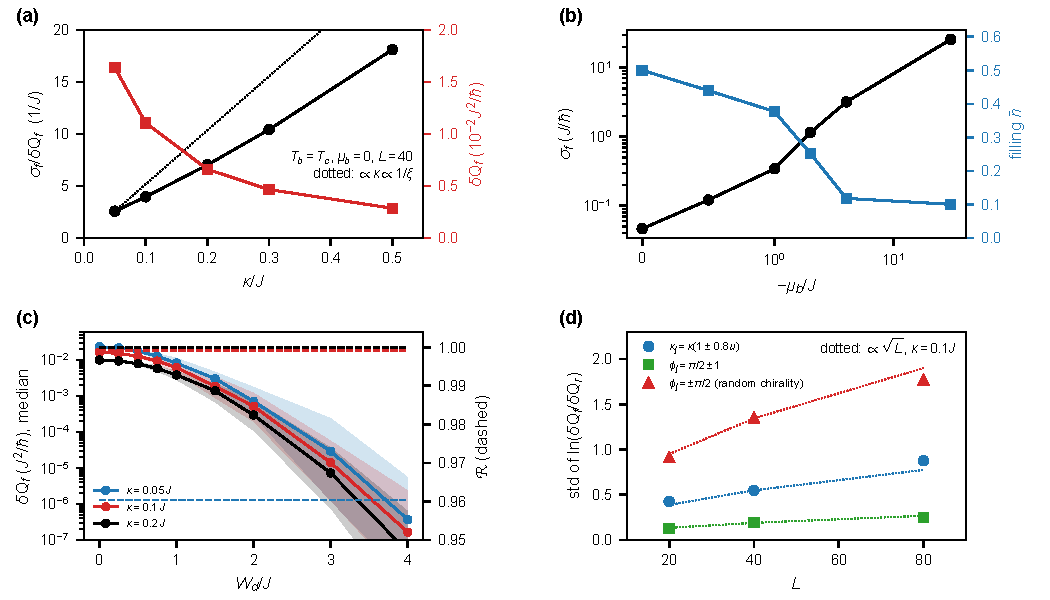
\includegraphics[width=0.78\textwidth]{fig4.pdf}
\caption{\textbf{Thermodynamic cost and robustness of skin-effect rectification.}
(a) Entropy produced per unit of rectified heat, $\sigma_f/\dQ_f$, when every bond is coupled to a thermal bath at $T_b=T_c$ and $\mu_b=0$ ($L=40$, mesoscopic leads and baths); it grows linearly with $\kappa\propto1/\xi$ (dotted line) while the throughput $\dQ_f$ (red) decreases.
(b) Entropy production and filling against the bath chemical potential for $\kappa=0.2J$; the ratio $\dQ_f/\dQ_r$ is identical ($\ln=14.23$) for all $\mu_b$ and $T_b$, but a particle sink ($\mu_b\to-\infty$) costs three orders of magnitude more entropy than a half-filled bath.
(c) On-site disorder of width $W_d$ ($L=40$, $60$--$100$ samples): the rectification $\R$ (dashed, right axis) is exactly sample independent, while the median forward throughput (solid, bands are the 10th--90th percentiles) collapses by Anderson localisation.
(d) Bond disorder ($\kappa=0.1J$): the standard deviation of $\ln(\dQ_f/\dQ_r)$ over samples grows as $\sqrt{L}$ in accordance with the sum rule of Eq.~(\ref{eq:sumrule}); only random chirality (red) destroys the rectification on average.
}
\label{fig4}
\end{figure*}

\textit{Thermodynamic cost.}---A pure loss channel is a reservoir at zero temperature and the entropy balance of the diode is then ill defined. To close it we replace each $L_j$ by a mesoscopic bath of $K_b$ modes at $(T_b,\mu_b)$ coupled through the same bond operator $c_j+e^{i\phi}c_{j+1}$ with damping rate $\kappa$, so that detailed balance holds and the entropy production $\sigma=-\sum_\alpha(\dot E_\alpha-\mu_\alpha\dot N_\alpha)/T_\alpha\ge0$ is defined for all reservoirs $\alpha$ (SM, Sec.~S5). Two results follow.
First, the ratio $\dQ_f/\dQ_r$ is exactly independent of $(T_b,\mu_b)$, because both responses are linear in the lead distributions and the bath contribution cancels in the difference; numerically the ratio agrees to $10^{-9}$ for $T_b=0.25J$--$2J$ and $\mu_b=0$ to $-30J$ [Fig.~\ref{fig4}(b)]. The dissipator fixes the nonreciprocity; the occupation of the bath only fixes its cost. The discreteness of the bath renormalises $t_\pm(\varepsilon)$ slightly, and the law is recovered in the wide-band limit (SM, Sec.~S5).
Second, with all baths at the cold temperature the isothermal state produces no entropy, so $\sigma_f$ is the entropy production of the rectification process itself. It is nearly independent of $\kappa$ ($0.042$--$0.052\,J/\hbar$ for $\kappa=0.05J$--$0.5J$), whereas $\dQ_f$ falls, so the entropy produced per unit of rectified heat grows as $\sigma_f/\dQ_f\propto\kappa\propto1/\xi$ [Fig.~\ref{fig4}(a)]. The cost is the heat that leaks from the hot lead into the bulk bath; the diode works at half filling with no particle current when $\mu_b=0$, whereas operating it as a particle sink ($\mu_b\to-\infty$) drains the chain and multiplies $\sigma_f$ by $500$ for the same ratio [Fig.~\ref{fig4}(b)]. We also find the exact identity $\sigma_f(T_b=T_c)=\sigma_f(T_b=T_h)$, a consequence of the fact that mirror reflection maps $\heff$ to its transpose, so that the two end reflectances are equal although $G_{L1}\neq G_{1L}$ (SM, Sec.~S2).

\textit{Robustness.}---Because Eq.~(\ref{eq:law}) involves no diagonal element of $\heff$, on-site disorder of any strength and distribution leaves $T_{RL}(\varepsilon)/T_{LR}(\varepsilon)$, $\dQ_f/\dQ_r$ and $\R$ exactly unchanged, sample by sample, even deep in the Anderson-localised regime where the throughput has collapsed by five orders of magnitude [Fig.~\ref{fig4}(c)]. The rectification is thus independent of eigenstate localisation, which affects both directions equally; the only experimental requirement is a usable throughput, $W_d\lesssim2J$ for $\dQ_f\gtrsim10^{-3}J^2/\hbar$. Bond disorder, $\kappa_j$ and $\phi_j$ varying from bond to bond, obeys the sum rule
\begin{equation}
\ln\frac{\dQ_f}{\dQ_r}=2\sum_{j=1}^{L-1}\ln\Bigl|\frac{t_{-,j}}{t_{+,j}}\Bigr|,
\label{eq:sumrule}
\end{equation}
so the exponent is a sum of independent bond contributions: it is self-averaging, with sample-to-sample fluctuations $\propto\sqrt{L}$ and a relative width that vanishes for long chains [Fig.~\ref{fig4}(d)]. A spread of loss rates leaves the mean unchanged ($7.85$ against the clean $7.81$ for $L=40$); a spread of phases rescales it by $\langle\sin\phi_j\rangle$; only random chirality, $\phi_j=\pm\pi/2$ with equal probability, gives a mean of zero and a rectification direction that is random from sample to sample. With $t_2\neq0$ the on-site invariance is lost but the ratio changes by less than $10\%$ for $W_d\le2J$ (SM, Sec.~S6).

\textit{Experimental realisation.}---The bond loss of Eq.~(\ref{eq:Lj}) follows from coupling neighbouring sites to a strongly damped auxiliary mode, $g(c_j^\dagger a_j+e^{i\phi}c_{j+1}^\dagger a_j+{\rm h.c.})$ with decay rate $\Gamma_a\gg g$, giving $\kappa=4g^2/\Gamma_a$. In momentum-lattice Bose condensates a dissipative Aharonov--Bohm chain of exactly this type has produced the non-Hermitian skin effect~\cite{Liang2022}; with $J=2\pi\times0.5$~kHz, $\kappa/J=0.05$--$0.2$ requires $\kappa=2\pi\times25$--$100$~Hz, and $\R>0.99$ needs $L\simeq15$ sites at $\kappa/J=0.2$. Thermal leads are provided by the two-terminal geometry of cold-atom transport~\cite{Brantut2012,Krinner2017}, and $\dQ_{f,r}$ follow from the energy and atom-number changes of the reservoirs. In superconducting circuits ($J=2\pi\times10$--$50$~MHz) a low-$Q$ auxiliary resonator per bond with $\Gamma_a\sim2\pi\times10$~MHz and $g\sim2\pi\times1$--$3$~MHz gives $\kappa=2\pi\times0.5$--$2$~MHz, with thermal leads realised by noise temperatures of $20$--$300$~mK injected into the end transmission lines. The carriers are then photons, but Eq.~(\ref{eq:law}) is an identity of single-particle Green functions and holds for bosons with pure loss as well (SM, Sec.~S2). Skin effects have so far been reached in superconducting hardware through squeezing in multimode cavities~\cite{Busnaina2024} and by post-selection on digital processors~\cite{Shen2025}; a loss-engineered Liouvillian skin effect in a circuit has not been reported, although its photonic counterpart has~\cite{Yang2026}, and the heat diode proposed here is a natural first target for one. Both platforms tolerate the site-to-site frequency disorder that is unavoidable in practice, because it does not enter Eq.~(\ref{eq:law}).

\textit{Conclusion.}---We have shown that a reciprocal chain with directional bond dissipation is a heat diode whose rectification ratio is fixed by one number, the Liouvillian skin length, through an exact exponential law, and we have mapped the law's domain of validity in four directions: beyond nearest neighbours, with interactions, with a thermal dissipator and with disorder.
Two trends organise the results. The exponent is a transport property of the dissipator: it is the non-Bloch localisation length at the transport energy, it is blind to the spectral winding number, to on-site disorder and to the bath occupation, and it is not renormalised by interactions up to $V=2J$. In contrast, every mechanism that makes the device less ideal acts on the prefactor: interactions, next-nearest hopping and Anderson localisation all lower the throughput and never the slope. Quantitatively, the ratio grows as $e^{2(L-1)/\xi}$ and reaches $\R>0.99$ at $L/\xi\simeq3$, two orders of magnitude beyond the size-independent ratios of nonlinear thermal rectifiers~\cite{Li2012}, and the price is an entropy production per rectified heat of order $\kappa$.
These results place skin-effect transport in the same category as topological edge transport: a directional response set by a bulk length rather than by local details, with disorder affecting only the magnitude. They also carry a warning for experiments on dissipative lattices: a heat or particle current asymmetry that is not measured as a function of length cannot be attributed to the skin effect, because the prefactor is model dependent while only the exponent is universal, and the entropy budget must be measured against the bath occupation and not against the loss rate alone. Two questions remain open: whether the slope stays unrenormalised for interactions strong enough to drive the chain into a correlated insulator, and whether the identity $\sigma_f(T_c)=\sigma_f(T_h)$ reflects a fluctuation relation for Liouvillian skin systems. Engineered dissipation is now routine in cold atoms and circuits, and the law derived here gives a direct, size-resolved test of whether a dissipative lattice rectifies heat for the right reason.

\begin{acknowledgments}
Matrix-product-state simulations used TeNPy~\cite{Hauschild2018}.
\end{acknowledgments}

\section*{Data availability}
The data shown in all figures, the \texttt{skinheat} package that produced them, the matrix-product-state time series and the scripts that regenerate every figure from the stored data files are openly available at Zenodo (concept DOI to be inserted upon acceptance).

\bibliographystyle{apsrev4-2}
\bibliography{refs}

\end{document}
